The discovery of penicillin shortly before the Second World War has revolutionized human medicine in the western world by saving the lives of millions of soldiers and civilians \cite{cdc_biggest_2019}. It also made major advances in surgery possible \cite{worldwar_resistance}. Ever since then antibiotics play a very important role in our well established health system and we are depending on those drugs in order to fight bacterial infections.\\
Because of the positive experiences people made with penicillin they quickly started to use this compound in an irresponsible way. This led to a penicillin resistance within 32 years after it's discovery \cite{worldwar_resistance}.
Ever since then it was necessary to repetitively introduce new antibiotics to the market because bacteria evolved resistance against previously developed drugs. Therefor bacteria which are no longer susceptible to antibiotics are nothing new, the response of resistance to antibiotics has its roots as deep as the discovery of antibiotics itself. 

\section{Cause and urgency of antibiotic resistance}
In the last few decades a gap opened between the increased use of antibiotics and the decreased development of new drugs \cite{ventola_antibiotic_2015}.\\
Based on this imbalance antibiotic resistance emerged and nowadays causes a huge problem in the health sector.  
For example 1.6 € billion and 2.5 million additional hospital days were caused by resistant infections just for the European Union per year \cite{europaisches_zentrum_fur_die_pravention_und_die_kontrolle_von_krankheiten_bacterial_2009}. \\
Or it has been shown that methicillin-resistant Staphylococcus aureus kills more Americans each year than HIV/AIDS, Parkinson’s disease, emphysema, and homicide combined \cite{ventola_antibiotic_2015}.

Between 2000 and 2015 defined daily does of antibiotics increased by 65 \% which demonstrates the tremendous increase of antibiotic consumption \cite{klein_reply_2018}.
This huge increase over the last two decades is terrifying since it's common sense that this is pushing antibiotic resistance even further.\\
Surprisingly a big share of antibiotic consumption is unnecessary and irresponsible. Mainly two fields of heavy antibiotic consumption exists and waste of antibiotics take place in both of them.
One field is the health sector where a questionalbe amount of prescriptions happen.
Alone in the US approximately 50 \% of antibiotics are prescribed unnecessarily \cite{sharma_antimicrobial_2011}. This is mainly because of inaccurate identification of pathogens which could be heavily improved by introducing molecular diagnostic techniques such as PCR \cite{ventola_antibiotic_2015}. \\
The other field is the globally operating food industry. It's estimated that in the early 2000s 25-50 \% of all antibiotic consumption has it's source in the food industry \cite{palumbi_humans_2001}. What makes this extremely high use even less understandable is the fact, that most of the antibiotics are used prophylactic and to stimulate growth and not in order to cure sick animals.

Now that we have seen the perspective of consumption of antibiotics, it's time to look at the development site of antibiotics.\\
As seen earlier the global demand of antimicrobials is extremely high, which is why it's surprisingly that the development of antibiotics decreased significantly. For example 19 antibiotics were approved in 1980-1984. In 2010-2014 only six drugs were approved \cite{ventola_antibiotic_2015}. This observation is not biased by the sampling time but is a tendency which is ongoing since the last three decades. \\
The little interest in the pharmaceutical industry is caused by the cycle of fighting newly formed resistance with novel drugs itself. Newly approved antibiotics are usually held in reserve and only prescribed for infections that more established antibiotics can't treat. This policy helps to delay the emergence of resistant strains, but it also limits the investment in return \cite{fair_antibiotics_2014}. Another reason is that other drugs  are used to treat chronic ailments, antibiotics on the other hand are only used for a short time making them a lot less profitable \cite{fair_antibiotics_2014}. 0.5 billion \$ \cite{costs} is the estimated cost of the development for a novel antibiotic. Considering the reasons mentioned above, such development is seen as a very risky investment \cite{fair_antibiotics_2014}.

Because of the increase of consumption and the lack of development of antibiotics several resistant bacterial pathogens established themselves in recent times. 
Among gram-positive bacteria resistant Staphylococcus aureus currently poses the biggest threat \cite{ventola_antibiotic_2015} as mentioned above causing a severe number of deaths. The threat coming from gram-negative pathogens is even more frightening because many emerged multi drug resistance, making it almost impossible to treat infections caused by such pathogens. Common representatives of gram-negative resistant bacteria are Klebsiella pneumoniae, Pseudomonas aeruginosa, Acinetobacter \cite{ventola_antibiotic_2015} and extended spectrum \textbeta-lactamase (ESBL) producing Escherichia coli \cite{fair_antibiotics_2014}.\\
Since those pathogens listed above and others are becoming more frequently resistant to drugs of last resort the WHO published a list of priority pathogens. This list should encourage development of new antibiotics against pathogens published with this list \cite{noauthor_who_nodate}.\\
Understanding how much antibiotics are prescribed unnecessarily and how irresponsible they are used in the food industry, it's quite obvious that one key of managing resistant pathogens is to stop this extensive overuse. In human medicine new guidelines and methodologies have to be developed which help doctors in the decision whether it's necessary or not to prescribe antibiotics. New guidelines also have to be established in the food industry limiting this excessive prophylactic overuse. \\
Furthermore the development of antibiotics has to be pushed ether by governmental founding/rewards or pharmaceutical companies have to come up with new business models, making the development of antibiotics more profitable.
\newpage

\section{Antibiotics and mechanisms of resistance}
During the 21st century different classes of antibiotics were discovered and developed. All of them have in common, that they intend to harm the bacterial pathogen, without harming the patient. This is possible by targeting bacteria specific target sites. Such targets are often involved in the synthesis of molecules which are essential for the bacterial cell. 
For example tetracyclines inhibit bacterial protein synthesis by binding to 30S ribosomal subunit \cite{noauthor_mechanism_nodate}. Other mechanisms are inhibiting bacterial transcription by blocking the process of unwinding of the bacterial DNA (quinilones) or by inhibitting the folic acid metabolism which is targetd by suflonamides \cite{noauthor_fig._nodate}. 
The most common target is cell wall synthesis, since the cell wall is very specific for prokaryotes. \textbeta-lactams, a class of antibiotics to which also penicillin belongs, target mechanisms in cell wall synthesis. They are the most prescribed antibiotics in human medicine. That's also why a lot of resistant bacterial pathogens are resistant against members of this class of antibiotics \cite{noauthor_high_nodate}. Since with this thesis I'm foucins on resistance against \textbeta-lactams with cephalosporins in particular, I only describe the mechanism of action for this class of antibiotics. 

\subsection{Development and mechanism of action of \textbeta-lactams}

\textbeta-lactam antibiotics act by inhibiting the synthesis of the peptidoglycan layer of bacterial cell walls \cite{noauthor_-lactam_2019}. This is a very effective target, since peptidoglycan plays a fundamental role in the cell wall structure. A damaged cell wall leads to bursting of the cell caused by the osmotic pressure from the cytoplasm. This implements that gram-positive bacteria are especially vulnerable to \textbeta-lactams because the peptidoglycan forms the very outer layer of their cell membrane \cite{graevemoore_english:_2008}.\\
In detail the inhibition of peptidoglycan synthesis happens becuase the \textbeta-lactams are analogues of the amino acid D-alanyl-D-alanine \cite{fisher_bacterial_2005}. Those tow amino acids form the terminal residues of the NAM/NAG-peptides which are subunits of the peptioglycan layer \cite{fisher_bacterial_2005}. Those subunits are crosslinked to peptidogylcan by DD-transpeptidases. Now the \textbeta-lactams also bind to the DD-transpeptidases but they heavily inhibit its activity, which means that the NAM/NAG-peptide subunits are no longer crosslinked \cite{fisher_bacterial_2005}. Because \textbeta-lactams bind to those DD-tranpspeptidases those enyzmes are also called penicillin binding proteins, coming from penicillin being the most famous representative of \textbeta-lactams \cite{fisher_bacterial_2005}.

All of the \textbeta-lactams feature the reactive \textbeta-lactam ring, which is a highly strained and reactive cyclic amide. In general five groups of \textbeta-lactams can be classified. Those being penams, penems, carbapenems, monobactams and the cefems \cite{beta-lactam_nodate}. The classification is done by subgrouping their ring system which is responsible for the antimicrobial action \cite{fernandes_-lactams:_2013}. 
Cephalosporins belonging to the cephems are very important because they showed to be very potent and well tolerated by patients thus they are widely used antibiotics \cite{dancer_problem_2001}. Furthermore Cephalosporins can be divided into five generations which is mostly done based on the time-point of development. \\
First-generation cephalosporins are very active against gram-positive cocci but other than cefazolin which is used for surgical propyhlaxis this generation of drugs in not prescribed often anymore \cite{fernandes_-lactams:_2013}. The second generation of cephalosporins are all active against bacteria covered by first-generation drugs, but have extended coverage against gram-negative bacteria \cite{fernandes_-lactams:_2013}. The tendency of enhanced activity against gram-negative bacteria is further visible in third-generation cephalosporins. A common representative of this generation is ceftazidime \cite{klein_third-generation_1995}. Only two beta-lactams are classified under the fourth-generation of cephalosporins, those being cefepime and cefpirome \cite{fernandes_-lactams:_2013}. They were developed because bacterial pathogens started to gain resistance against third generation cephalosporins. 
The newest fifth generation of caphalosporins were explicitly developed to target resistant strains of bacteria but unfortunatley drugs belonging to this generation are ineffective against enterococci bacteria \cite{fernandes_-lactams:_2013} 

Penams are a large group of \textbeta-lactmas that include penicillins which are characterized by a basic bicyclic structure \cite{beta-lactam_nodate}. \\
Unlike penams, monobactams have a momocyclic \textbeta-lactam ring and are only active against gram-necative bacteria \cite{fernandes_-lactams:_2013}. Lastly carbapenems are also belonging to \textbeta-lactams and they have good activity against many gram-negative bacteria \cite{beta-lactam_nodate}.  

\subsection{Resistance mechanisms against \textbeta-lactams}

Because the \textbeta-lactam ring in \textbeta-lactam antibiotics is very reactive several enzymes are expressed in bacteria which are able to hydrolyze the \textbeta-lactam ring \cite{noauthor_beta-lactam_nodate}. This same ring is also involved in binding to the penicillin binding proteins and therefor hydrolyzed \textbeta-lactams are no longer bactericide \cite{noauthor_beta-lactam_nodate}. Those enzymes called \textbeta-lactamases were found before treatment of infections with \textbeta-lactams, because they occurred naturally in bacteria being exposed to bactericides produced from fungi \cite{noauthor_fig._nodateflem}.   

\subsubsection{\textbeta-lactamases}
Nowadays mainly plasmid-mediated \textbeta-lactamases are important because they can be easily transmitted via horizontal gene-transfer \cite{munita_mechanisms_2016}.  
The first plasmid-mediated \textbeta-lactamase in gram-negative bacteria was described in the early 1960s and called \textbeta-lactamase TEM-1 \cite{fernandes_-lactams:_2013}. Because its position on a plasmid and being transposon mediated, TEM-1 was found worldwide only few years later after it's first isolation \cite{fernandes_-lactams:_2013}. TEM-1 was able to cause resistance against \textbeta-lactams of this time.  That's why third-generation cephalosporins such as ceftazidime were developed which can't be hydrolyzed by TEM-1 \cite{fernandes_-lactams:_2013}. Those newly developed extended spectrum cephalosporins where thus heavily used exposing evolutionary formed variants of TEM-1 to selection \cite{fernandes_-lactams:_2013}. This caused further resistance against those newly developed extended cephalosporins \cite{fernandes_-lactams:_2013}. 
Another anciently known \textbeta-lactamase is called SHV-1 which was isolated for the first time in 1974 \cite{kuzin_structure_1999}. It's encoded chromosomally in the majority of isolates of K. pneumoniae but is also plasmid mediated when present in Escherichia Coli \cite{kuzin_structure_1999}. \\
\textbeta-lactamases which are able to hydrolyze extended-spectrum cephalosporins are called extended-spectrum \textbeta-lactamases or ESBLs. 

\subsubsection{Extended spectrum \textbeta-lactamases (ESBLs)}
Next to the TEM and SHV families new \textbeta-lactamases were isolated over the time of the last couple decades. One of them is called CTX-M-1 \textbeta-lactamase which was clinically isolated for the first time in Germany in 1986. It's name comes from the high affinity to cefotaxime \cite{fernandes_-lactams:_2013}. Because it only has a sequence identity of 40 \% compared to TEM or SHV \cite{bradford_extended-spectrum_2001} it got categorized as a new \textbeta-lactamase family. Later on many variants were isolated and the CTX protein family was subdivided into five subgroups, with CTX-M-1 being one of them  \cite{fernandes_-lactams:_2013}.
It's assumend that they evolved from the \textbeta-lactamase precursor AmpC from Klyzvera ascorbata  \cite{bradford_extended-spectrum_2001}. Even though the first CTX-M-1 was isolated in Germany, it's mostly popular in eastern Europe, South America and Japan \cite{bradford_extended-spectrum_2001}. \\
Another \textbeta-lactamase family belonging to the ESBLs is called OXA.
The OXA family was originally created as a phenotypic rather than a genotypic group, based on a specific hydrolysis profile \cite{bradford_extended-spectrum_2001}. Therefor the sequence identity compared to other members of this family is only about 20 \% \cite{bradford_extended-spectrum_2001}. It's name comes from the ability to efficiently hydrolyze oxacillin \cite{bradford_extended-spectrum_2001}.
\label{section:esbls}

\subsection{General resistance mechanisms}
\label{section:resistance_mechanisms}
By hydrolyzing \textbeta-lactams we have seen one strategy of bacterial resistance against antibiotics. There are other more general mechanisms which protect the pathogen form bactericide effects of antibiotics. \\
Another pathway of resistant bacteria is to decrease the antibiotic penetration and to increase efflux. That makes a lot of sense, because many antibiotics have targets which are located intracellularly \cite{munita_mechanisms_2016}. This implies that bacterial pathogens came up with pathways which are making it more difficult for the antibiotic to reach the cytoplasm, or they introduced pathways which actively transport the antibiotic out of the cell. Some compounds such as \textbeta-lactams rely on channels in the membrane of the bacteria called porins, because they are hyrdophylic and therefor can not just pass the lipophylic membrane by diffusion \cite{munita_mechanisms_2016}. This gives the bacteria the opportunity to reduce the numbers of porins or to change their structure \cite{munita_mechanisms_2016}. It's noteworthy that changing permeability is an especially effective strategy for gram-negative bacteria to protect themselves from \textbeta-lactams. That's because the \textbeta-lactams have to cross the outer membrane in order to inhibit the peptidoglycan synthese \cite{munita_mechanisms_2016}. \\
It's much more complicated on the other hand to produce efflux pumps, which actively transport the toxic compoud out of the cell. One of the earliest described efllux pump system are the Tet efflux pumps which are using proton exchange as source of energy \cite{munita_mechanisms_2016}.\\
Another mechanism is changing of the target site. Some antibiotics such as rifampin binds to a very conserved pocked within the RNA polymerase of the bacteria. Now by chromosomal mutations coding for this RNA polymerase the bacteria changed the structure of this pocket and therefor they were no longer susceptible to rifampin \cite{munita_mechanisms_2016}.    

\section{An overview of antibiotic resistant pathogens in Switzerland}
\begin{figure}
	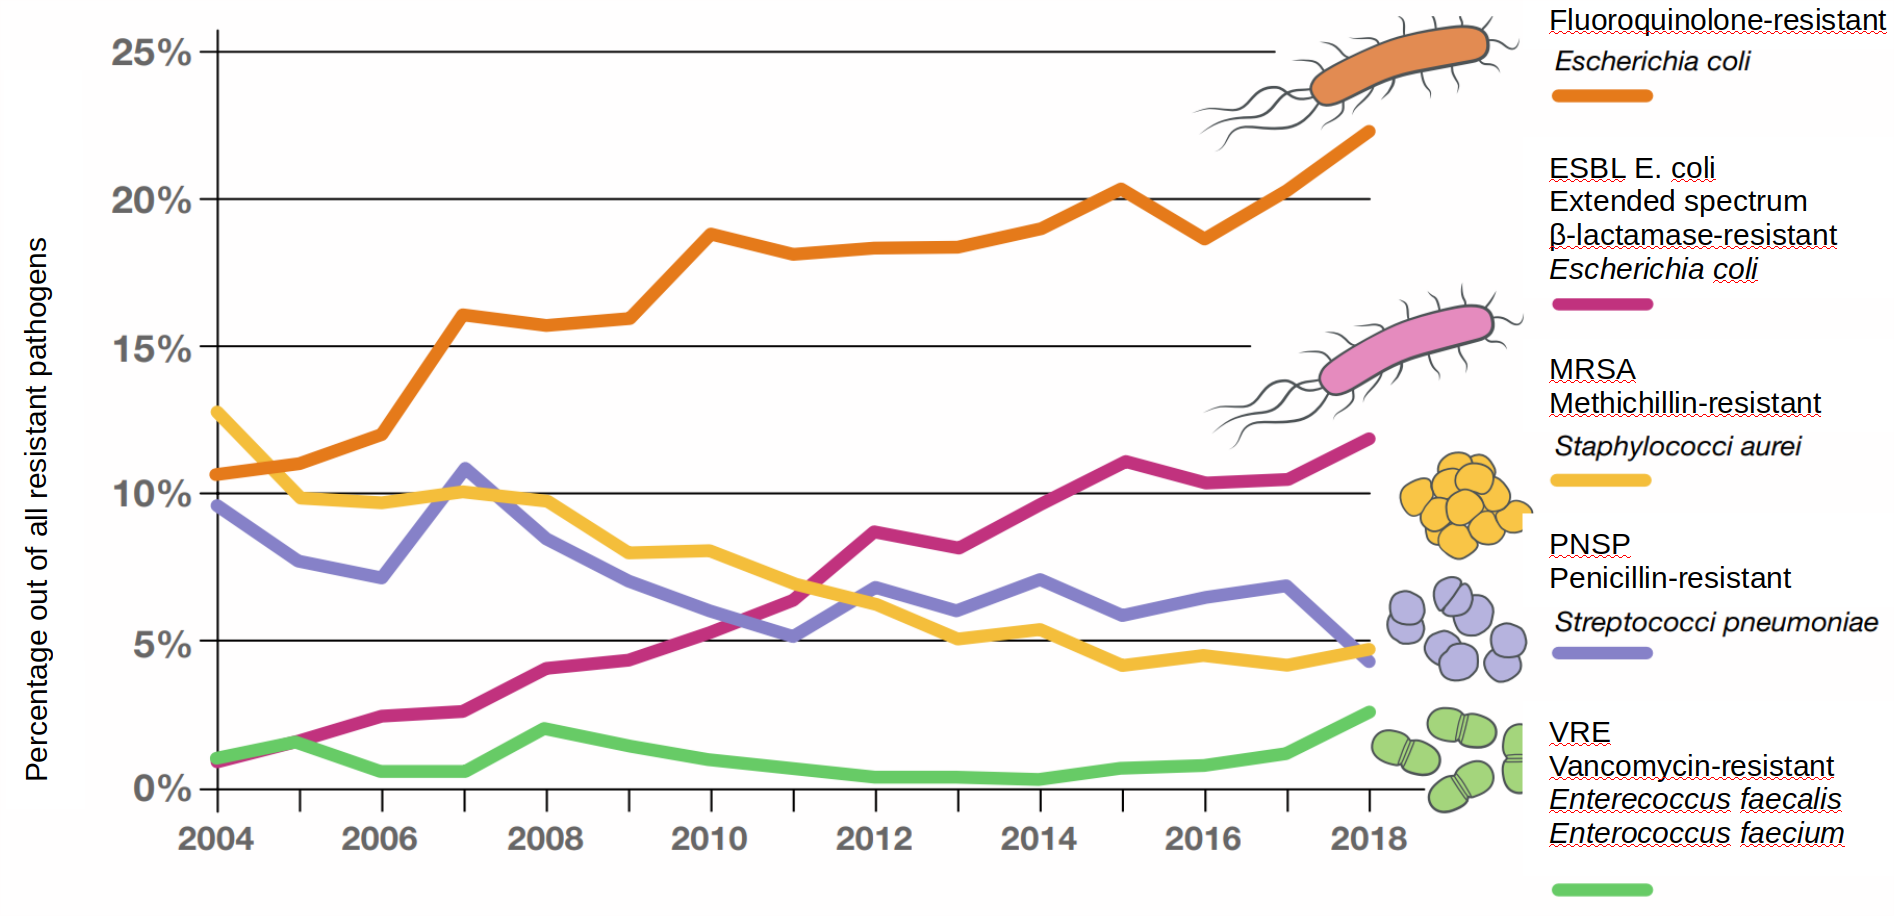
\includegraphics[scale=0.2]{pathogens_overview.png}
	\caption{Development of popularity of antibiotic resistant pathogens.
		\cite{swiss_hospitals_pathogens}}
	\label{figure:pathogen_dvelopment}
\end{figure}

For Switzerland the rate of antibiotic consumption divided by the Swiss population stayed the same in recent times, but the absolute consumption increased too. This is because more people were getting treated in hospitals \cite{swiss_hospitals} but the general population of Switzerland increased too.

The biggest challenge with resistant pathogens in Switzerland is ongoing in hospitals where yearly 300 people die because of infections with antibiotic resistant bacteria \cite{noauthor_fast_2018}. Hospitals are often hot-spots of resistant bacteria because there is a high density of  pathogens, combined with high locally applied antibiotic doses. This generates an increased antibiotic pressure and selection. Unfortunately many patients have a weakened immune system making them a lot more vulnerable to infections with antibiotic resistant bacteria.


Mainly five strains which cause problems in treatment with antibiotics are present in Swiss hospitals. Their increasing or decreasing spread can be seen in Figure \ref{figure:pathogen_dvelopment}\cite{swiss_hospitals}. 

\textbf{Staphylococcus aureus} is a gram-positive bacterium which is normally present in the upper respiratory tract and on the skin. As a pathogen Staphylococcus aureus can cause skin and bone inflammations and is responsible for the most inflammations of surgical wounds \cite{tong_staphylococcus_2015}. The most common resistance formed by S. aureus is resistance against an antibiotic called methicillin, a penicillin like compound. Resistance is achieved by those pathogens by expressing a gene coding for for a penicillin binding protein PBP2a which has significantly lower affinity to \textbeta-lactams \cite{peacock_mechanisms_2015}.  There are compounds which effectively kill this certain pathogen but resistance against such compounds have been reported already \cite{ventola_antibiotic_2015}. As seen in Figure \ref{figure:pathogen_dvelopment} there is a decrease of this pathogen which could mainly be achieved by aggressive preventive hygiene measures in hospitals and improved screening for this pathogen \cite{ventola_antibiotic_2015}\cite{swiss_hospital}. 

\textbf{Streptococcus pneumoniae}, a gram-positive bacteria, is normally present in the nose and throat of most individuals \cite{ventola_antibiotic_2015}. But when Streptococcus pneumoniae turns into a pathogen, which mainly happens in elderly patients, it causes severe blood and pulmonary infection causing around 7000 deaths per year \cite{ventola_antibiotic_2015e}. Usually resistant S. pneumoniae are not susceptible to penicillin like antibiotics by a similar mechanism as described for S. auresus (mutations in the penicillin binding proteins). Visible in Figure \ref{figure:pathogen_dvelopment}, this pathogen is decreasing as well, which is mainly because of the introduction of the PCV7 vaccine. This vaccine provides protection against several pneumococcal strains, which reduces the transmission of resistance \cite{ventola_antibiotic_2015}. 

\textbf{Enterococci} such as Enterococcus faecalis are responsible for a rather small share of resistant pathogens as visible in Figure \ref{figure:pathogen_dvelopment}. Unfortunately it's very difficult to treat this gram-positive bacteria because only very few antimicrobial options are available \cite{ventola_antibiotic_2015}. This pathogen is so hard to treat because it developed several pathways of mechanism. Modifications in penicillin binding proteins, over-expression of efflux pumps and a cell response that promotes survival in the human host \cite{miller_mechanisms_2014}.

\textbf{Escherichia coli} belongs to the enterobacteriaceae and is present in every intestine as a gram-negative bacterium. However they are able to cause infections when present in other parts of the body leading mainly to infections of the urinary tract but also in the brains of new borns \cite{swiss_hospitals_pathogens}. Traditionally treatment of E. coli was successful by applying doses of third-generation cephalosporines. In the last two decades E. coli started to gain resistance against such extended \textbeta-lactams by producing extended spectrum \textbeta-lactamases (also see section \ref{section:esbls}). As seen in Figure \ref{figure:pathogen_dvelopment} in 2004 only 1 \% of of resistant pathogens in Swiss hospitals were ESBL prodcuing E. coli. 14 years later they were already responsible for 14 \% of infections with resistant pathogens. Luckily ESBL producing E. coli are still susceptible to carbapenems but other bacterial strains already developed resistance against carbapenems \cite{noauthor_treatment_nodate}. That's why carbapemen should only be used as a very last option of treatment of ESBL E. coli infections, because chances are quite high, that they are able to evolve resistance against this compound too by for example picking up genes by horizontal gene transfer coding for carbapenemases which are able to hydrolyze crabapenem.  \cite{ventola_antibiotic_2015}. 


\section{ESBL E. coli}
Since by now ESBL E. coli can still be treated with antibiotics of last resort such as carbapenems it's extremly important to use those drugs with high awareness. Therefor institutions such as the EUCAST came up with guidelines in order to assist clinical microbiologist in making the right decision in prescribing adequate antibiotics \cite{leclercq_eucast_2013}. The EUCAST is also responsible for defining breakpoints. This means they publish data defining which concentration has to be exceeded in order that a certain pathogens is seen as resistant against a specific antibiotic \cite{leclercq_eucast_2013}. \\
In the past when it was determined that an infection is caused by E. coli, the strain was cultured and susceptibility was tested by determining the MIC. Additionally presence or absence of an ESBL genes was tested by molecular characterisation \cite{kahlmeter_breakpoints_2008}. Such molecular characterisation was typically done by PCR or microarrays \cite{arlet_molecular_1995}. Now when ether the determined MIC was above the breakpoint defined by the EUCAST or the molecular characterisation showed positive results for ESBLs, carbapenemes were described. But it was shown, that sometimes the MIC was below the breakpoint even though ESBLs were detected. Prescribing antibiotics of last resort in such cases was therefor proven to be unnecessary and wrong. As a reaction EUCAST corrected their guidelines and now just susceptibility by MIC determination is considered for making the decision which antibiotic should be prescribed \cite{leclercq_eucast_2013}. Unfortunately MIC determination takes about 48 hours which is too long in some cases forcing prescription of carbapenemens even though it's unknown if it's actually necessary.\\
Completely ignoring genomic data seams not ideal, because chances are quite high that whether E. coli which have ESBL genes are resistant or not is encoded in the genome. This just means that other characteristics have to be defined, since it's not sufficient to simply look if genes coding for ESBLs are present.

\section{Studying differences in the genome between extended cephalosporine susceptible and resistant E. coli}
Some resistant mechanism as for example a change in the target binding site, rely on mutations and therefore imply a change in the genome. Other examples for resistance based on mutations are a different structure of porins making the membrane less permeable for \textbeta-lactams, or a change in the structure of efflux pumps which may changes the affinity for a certain substrate. Other mechanisms could rely on up-regulation, which could have its source in a mutation in a promoter region. \\
As by now it was assumed that the resistance of ESBL E. coli is based on the expression of ESBLs, which are able to hydrolyze \textbeta-lactams \cite{shaikh_antibiotic_2015}. But as described earlier some E. coli which have ESBL coding genes are not resistant. This could mean that extended cephalosporine susceptible E. coli which have ESBL genes are not actually expressing such \textbeta-lactamases. This could be clarified by studying the ESBL protein levels for susceptible and resistant ESBL E. coli. It's also possible, that other resistant mechanisms other than hydrolysis of the compound have an impact on susceptibility.\\
Ether if a change in the expression levels or other mechanisms are responsible for the resistance, it's quite possible that at least a part of the resistance is based on mutations. Those mutations could be identified by comparing the genomes of susceptible and resistant E. coli. \\
Our goal is to identify such mutations which could be involved in the resistance. In order to do so, we pursue two different approaches. One of them is study the genomes of clinical samples of ESBL E. coli which are provided by our collaborator who is the head of clinical microbiology at the University hospital of Basel. He took samples of patients who were infected with E. coli where ESBLs were detected by PCR. Over the process of treatment he continously took samples and determined their susceptibility to cefepime and ceftazidime. This lead to a sample collecton of ESBL E. coli which were susceptible to extended cephalosporines but evolved resistance, or for some patients resistance was lost over time. By isolating the DNA and deep-sequencing all of the isolates, we identify SNPs in the resistant samples, which are potentially involved in the resistant mechanism. \\
For the other approach we assemble a system called morbidostat, which allows to automatically culture bacteria. The morbidostat is continiously recording the growth of the cultures and injects appropriate doses of antibiotics. This creates constant inhibition of the growth and forces resistance and selection. Along this pathway we want to take samples and deep-sequence the isolated DNA. Similar to analysis for the clinical samples, we want to identify mutations which accumulated over the time where the bacteria were forced to evolve resistance. \\
Both approaches rely on next generation sequecing technologies. 
To get the most accurate genomes we want to use two different next generation sequencing technologies.  

\subsubsection{Illumina and Nanopore sequning}
Illumina sequencing is a method which produces short reads which are typically 150 base pairs (bp) long. The strong-suit of Illumina sequecning is the low error rate which was dertermined as 0.24 \% per base \cite{pfeiffer_systematic_2018}. A common used Illumina sequecing system is the MiSeq-System which is also used for this project. The downside of this technology is that even though sequencing itself is rather cheap, the instrument costs are high. Furthermore Illumina sequecing has a tendency to generate more reads of GC-enriched DNA fragments \cite{noauthor_illumina_nodate}. Also it's not possible to assemble structurally correct whole-genomes, because the reads are short. 

Oxford Nanopore Technologies allows sequencing with very little laboratory equipment which is also coming with very low instrument costs. This technology produces very long reads which are up to several 100 kbp long. In contrast to Illumina sequencing the error rate per base is 13.6 \% \cite{noauthor_resolving_nodate} which is a lot higher. But because the reads are so long it's possible to assemble structurally correct whole-genomes. \\
By comparing both technologies, it's pretty obvious that their strong suits are quite contrary. Illumina produces short but accurate reads, Nanopore long and inaccurate reads. Since the costs of both techniques dropped tremendously over the last couple years, it's possible to sequence DNA isolates on both platforms and combine the output in one assembly which is called hybrid assembly. This has the benefit that the advantages of both platforms are combined, leading to assemblies with a low nucleotide error rate but also with high structural correctness.  \\


\subsection{Principles and experiences with the morbidostat} 
The morbidostat was initially invented by Toprak et al \cite{morb_toprak}. Later on Neher et al \cite{doselmann_rapid_2017} rebuilt the system in 2015. Based on those two systems we rebuild a morbidostat with small modifications which should improve the handling and mainly make it a lot more compact. This is important since we want to use the morbidostat in a space limiting hypoxi-station. \\
With the morbidostat 15 cultures can be grown independently in vials. Thereby the growth of each culture is monitored by measuring and saving the optical density (OD). As shown in the left Figure \ref{figure:vial_setup} measuring of the OD is done by detecting scattered light emitted by LEDs. Based on the growth an appropriate dose of antibiotics is calculated using a control algorithm and injected into the cultures. This leads to an inhibition of the growth without entirely killing ever colony forming unit. The appropriate dose of antibiotics is achieved by mixing different drug concentrations using computer controllable pumps which are also injecting the drug into the vials.
The morbidostat allows to study drug resistance evolution in real-time, while having an idea of the progress of evolution in resistance.

In the morbidostat, bacteria are grown in a fixed volume. The process of suppressing the growth with antibiotics is divided into cycles which are constantly getting executed. One cycle has following tasks and commands:
\begin{itemize}
	\item Measuring the OD every several seconds over a defined cycle time \textDelta t, which is typically 10 minutes 
	\item Calculating growth rate at the end of the cycle based on the previously collected ODs
	\item Based on growth, injection of appropriate dose of drug, as calculated by a feedback algorithm
	\item Remove excess volume (waste)
\end{itemize}
In the right Figure \ref{figure:vial_setup} three cycles are shown. Because under certain conditions fluid is getting injected, this leads to a dilution is visible in the OD at the start of the new cycle. \textDelta OD represents how fast the bacteria are grown. It's the difference of the optical densities from the end of two cycles.  
\begin{figure}
	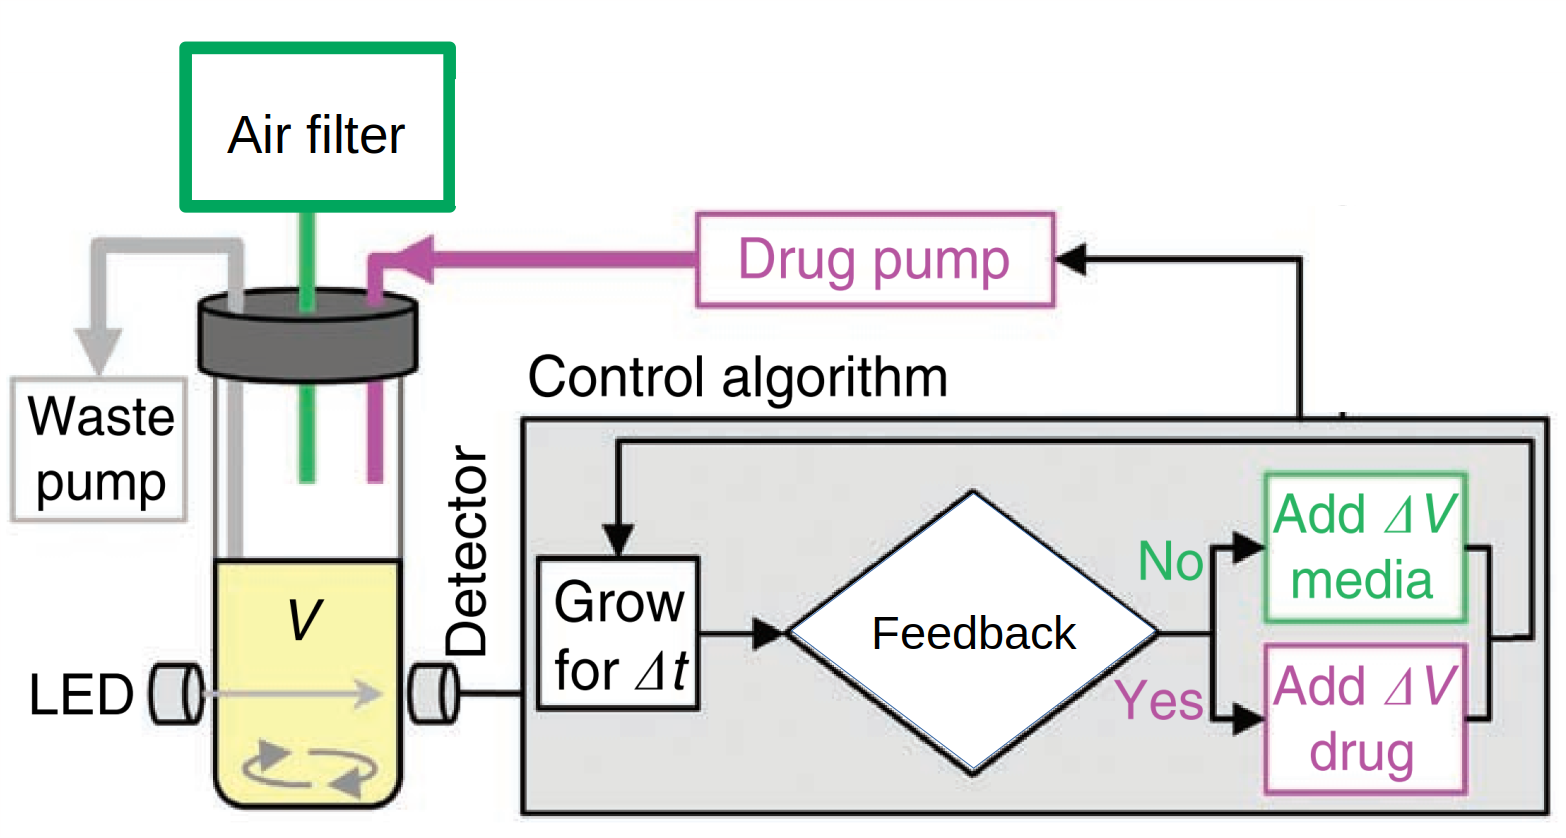
\includegraphics[scale=0.1]{vial_diagram.png}
	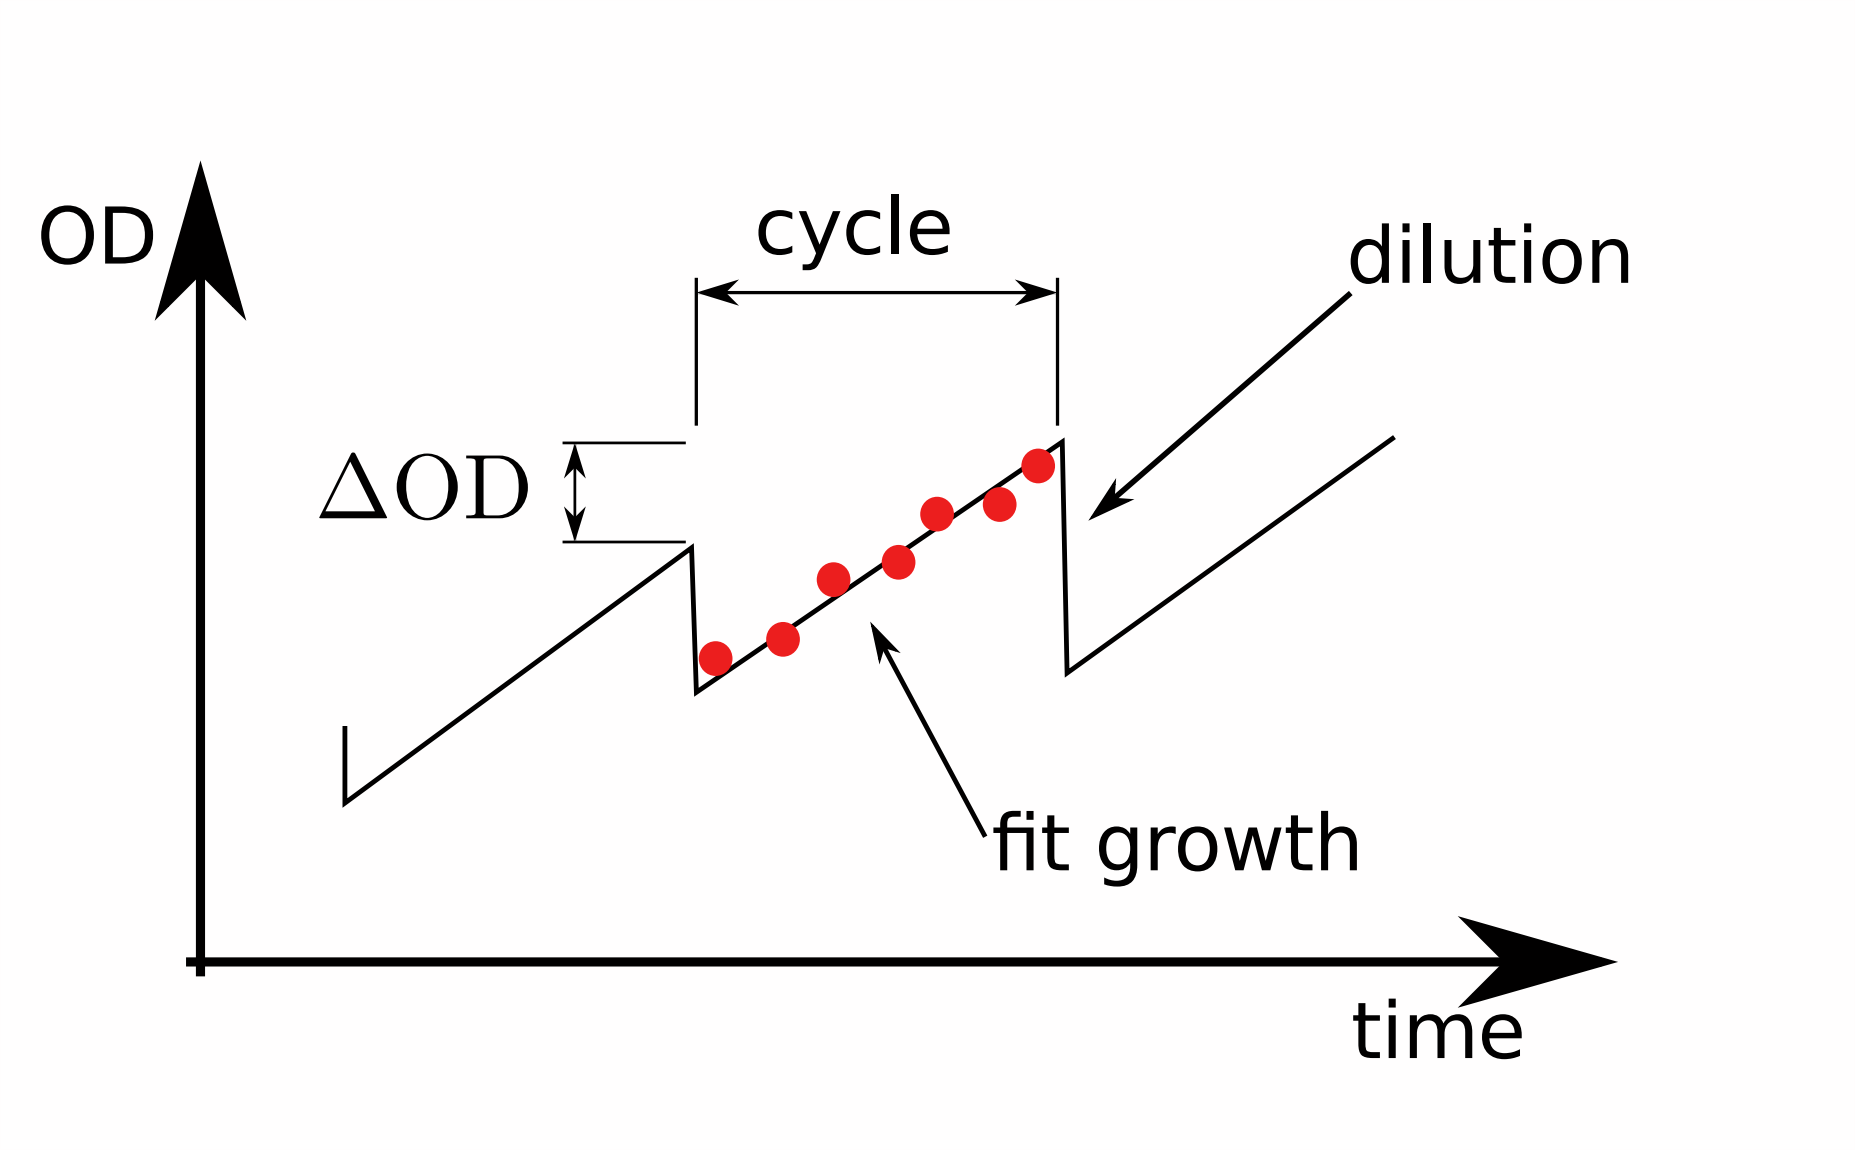
\includegraphics[scale=0.07]{growth_diagram.png}
	\caption{Based on the growth a feedback algorithm decides whether and how much drug is getting injected}
	\label{figure:vial_setup}
\end{figure}

\subsubsection{Previous morbidostat experiments and expected outcome}
Dösselmann et al \cite{doselmann_rapid_2017} used the morbidostat in order to study colistin resistance. With the morbidostat they were able to increase the MIC of colistin for Pseudomanas aeruginosa a 100-fold within 20 days \cite{doselmann_rapid_2017}. Along the evolutionary pathway they were able to identify a mutation pattern. The mechanism of action for colistin is to displace cations from the phospate groups of membrane lipids. This leads to disruption of the outer cell membrane causing cell death \cite{noauthor_colistin:_nodate}. Therefor it's not surprise that Bianca et al could identify several mutations coding fro proteins involved in the lipopolysaccharide synthesis \cite{doselmann_rapid_2017}. 
\\
The mutations that we find in the analysis form the clinical samples but also from the morbidostat experiment hopefully lead to a better understanding in the resistance mechanism of ESBL E. coli. Obviously the data has to be validated by for example  synthetically introducing mutations of interest to extended cephalosporine susceptible ESBL E. \\
The mutations can be used by our collaborator who is studying protein levels in ESBL E. coli. For example mutations found in promotor region can be compared to protein level expression data in order to tell if they have an impact on the expression.